% 2D domain decomposition into 2 x 2 subdomains with a one-cell halo (ghost) layer.
% Rank 0 shows its halo cells; arrows show the halo exchange with its neighbors.
% Set \n (cells per subdomain side) and the halo width with \h.
\documentclass[border=5pt]{standalone}
\usepackage{tikz}
\usetikzlibrary{arrows.meta}
\begin{document}
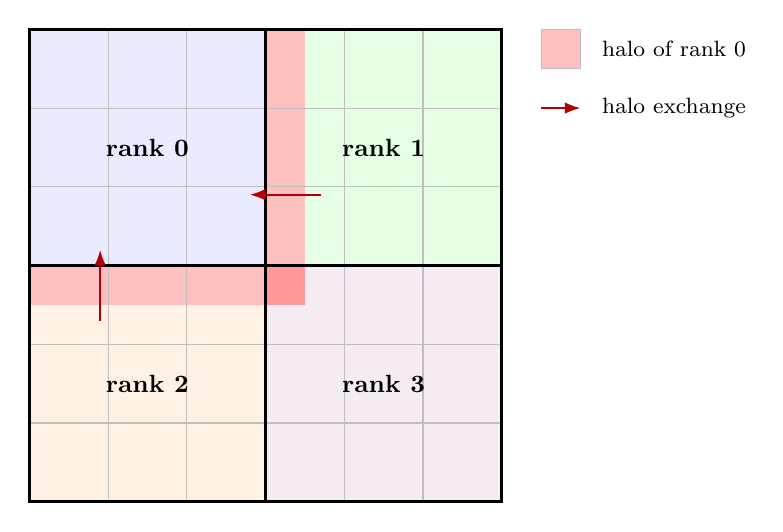
\begin{tikzpicture}[
    x=0.5cm, y=0.5cm,
    rank/.style={font=\small\bfseries},
    xch/.style={-{Latex[length=2mm]}, thick, red!70!black},
]
\def\n{6} % cells per subdomain side
\def\h{1} % halo width in cells
\pgfmathtruncatemacro{\N}{2*\n}
% Subdomain fills
\fill[blue!8]   (0,\n) rectangle (\n,\N);
\fill[green!10] (\n,\n) rectangle (\N,\N);
\fill[orange!10](0,0) rectangle (\n,\n);
\fill[violet!8] (\n,0) rectangle (\N,\n);
% Halo of rank 0 (top-left): cells of the neighbors that rank 0 copies.
% Right strip from rank 1, bottom strip from rank 2, corner cell from rank 3.
% A 5-point stencil needs only the two strips; a 9-point stencil also needs the corner.
\fill[red!25] (\n,\n) rectangle (\n+\h,\N);       % from rank 1
\fill[red!25] (0,\n-\h) rectangle (\n,\n);        % from rank 2
\fill[red!40] (\n,\n-\h) rectangle (\n+\h,\n);    % corner, from rank 3
% Cell grid
\draw[gray!50] (0,0) grid (\N,\N);
% Subdomain borders
\draw[very thick] (0,0) rectangle (\N,\N);
\draw[very thick] (\n,0) -- (\n,\N);
\draw[very thick] (0,\n) -- (\N,\n);
% Rank labels
\node[rank] at (\n/2,\n+\n/2) {rank 0};
\node[rank] at (\n+\n/2,\n+\n/2) {rank 1};
\node[rank] at (\n/2,\n/2) {rank 2};
\node[rank] at (\n+\n/2,\n/2) {rank 3};
% Exchange arrows
\draw[xch] (\n+\h+0.4,\n+\n/2-1.2) -- (\n-0.4,\n+\n/2-1.2);
\draw[xch] (\n/2-1.2,\n-\h-0.4) -- (\n/2-1.2,\n+0.4);
% Legend
\begin{scope}[shift={(\N+1,\N-1)}]
\fill[red!25] (0,0) rectangle (1,1); \draw[gray!50] (0,0) rectangle (1,1);
\node[anchor=west, font=\footnotesize] at (1.3,0.5) {halo of rank 0};
\draw[xch] (0,-1) -- (1,-1);
\node[anchor=west, font=\footnotesize] at (1.3,-1) {halo exchange};
\end{scope}
\end{tikzpicture}
\end{document}
